% THIS IS AN EXAMPLE DOCUMENT FOR VLDB 2012
% based on ACM SIGPROC-SP.TEX VERSION 2.7
% Modified by  Gerald Weber <gerald@cs.auckland.ac.nz>
% Removed the requirement to include *bbl file in here. (AhmetSacan, Sep2012)
% Fixed the equation on page 3 to prevent line overflow. (AhmetSacan, Sep2012)

\documentclass{vldb}
\usepackage{graphicx}
\usepackage{balance}  % for  \balance command ON LAST PAGE  (only there!)

\usepackage[printonlyused]{acronym}

\usepackage[backend=biber]{biblatex}
\bibliography{bibliography}

\newacro{TUB}{Berlin Institute of Technology}
\newacro{CIT}{Complex and Distributed IT-Systems}

\newcommand{\BigData}{\textsl{Big Data}}
\newcommand{\Stratosphere}{\textsl{Stratosphere}}
\newcommand{\map}{\texttt{map}}
\newcommand{\filter}{\texttt{filter}}
\newcommand{\reduce}{\texttt{reduce}}
\newcommand{\join}{\texttt{join}}
\newcommand{\groupby}{\texttt{groupby}}
\newcommand{\update}{\texttt{update}}
\newcommand{\storm}{\textsl{Storm}}
\newcommand{\ikeyconfig}{\texttt{IKeyConfig}}
\newcommand{\iwindow}{\texttt{Window}}
\newcommand{\ioperator}{\texttt{IOperator}}


\newcommand{\boldListItem}[1]
{
	\item{\textbf{#1:}}\hfill \\
}

\newcommand{\descriptor}[1]
{
	\item[#1:]\hfill \\
}

\newcommand{\keyword}[1]
{\texttt{#1}}


\begin{document}

	%
% paper title
% can use linebreaks \\ within to get better formatting as desired
\title{CIT-Storm\\ {\LARGE A Storm-based Big-Data Framework for Streaming Applications}}


% author names and affiliations
% use a multiple column layout for up to three different
% affiliations
\author{
\IEEEauthorblockN{Kay Fleischmann}
\IEEEauthorblockA{Berlin Institute of Technology\\TU-Berlin\\
				  10623 Berlin\\
				  Email: fleischmann.kay@gmail.com}
\and

\IEEEauthorblockN{Fridtjof Sander}
\IEEEauthorblockA{Berlin Institute of Technology\\TU-Berlin\\
				  10623 Berlin\\
				  Email: fsander@mailbox.tu-berlin.de}
\and

\IEEEauthorblockN{Gert Geidel}
\IEEEauthorblockA{Berlin Institute of Technology\\TU-Berlin\\
				  10623 Berlin\\
				  Email: gertimon@live.de}
\and

\IEEEauthorblockN{Michael Thomas}
\IEEEauthorblockA{Berlin Institute of Technology\\TU-Berlin\\
				  10623 Berlin\\
				  Email: michi.t@mailbox.tu-berlin.de}
\and

\IEEEauthorblockN{Thomas Misch}
\IEEEauthorblockA{Berlin Institute of Technology\\TU-Berlin\\
				  10623 Berlin\\
				  Email: thmis@mailbox.tu-berlin.de} 
\and

\IEEEauthorblockN{Constantin Gaul}
\IEEEauthorblockA{Berlin Institute of Technology\\TU-Berlin\\
				  10623 Berlin\\
				  Email: constantin.gaul@gmail.com}
}

% conference papers do not typically use \thanks and this command
% is locked out in conference mode. If really needed, such as for
% the acknowledgment of grants, issue a \IEEEoverridecommandlockouts
% after \documentclass

% for over three affiliations, or if they all won't fit within the width
% of the page, use this alternative format:
% 
%\author{\IEEEauthorblockN{Michael Shell\IEEEauthorrefmark{1},
%Homer Simpson\IEEEauthorrefmark{2},
%James Kirk\IEEEauthorrefmark{3}, 
%Montgomery Scott\IEEEauthorrefmark{3} and
%Eldon Tyrell\IEEEauthorrefmark{4}}
%\IEEEauthorblockA{\IEEEauthorrefmark{1}School of Electrical and Computer Engineering\\
%Georgia Institute of Technology,
%Atlanta, Georgia 30332--0250\\ Email: see http://www.michaelshell.org/contact.html}
%\IEEEauthorblockA{\IEEEauthorrefmark{2}Twentieth Century Fox, Springfield, USA\\
%Email: homer@thesimpsons.com}
%\IEEEauthorblockA{\IEEEauthorrefmark{3}Starfleet Academy, San Francisco, California 96678-2391\\
%Telephone: (800) 555--1212, Fax: (888) 555--1212}
%\IEEEauthorblockA{\IEEEauthorrefmark{4}Tyrell Inc., 123 Replicant Street, Los Angeles, California 90210--4321}}




% use for special paper notices
%\IEEEspecialpapernotice{(Invited Paper)}




% make the title area
\maketitle

	\begin{abstract}
%\boldmath
The abstract goes here.
\end{abstract}
	\section{Introduction}
\label{sect:introduction}

The amount of data stored world wide grows continuously -- \BigData\ is everywhere. The term \BigData\ refers to the practice of using large data sets from multifarious sources and processing them with high speed and efficiency to create valuable business information. Classical relational databases are often not capable of processing such large volumes of data. Thus, a new type of software is exploited by \BigData, that runs on hundreds or thousands of machines in parallel, like \Stratosphere\ by the \textsl{\ac{TUB}} or \textsl{Hadoop}, the open-source implementation of Map-Reduce. Until now, many recent platforms are restricted to process static data sets stored on distributed file systems. These system do not meet challenges of real-time processing tasks, that handle data streams generated by the world-wide-web or sensor networks.

The group \textsl{\ac{CIT}} at the \textsl{\ac{TUB}} aims to fill that gap by exploring how \BigData-platforms can be extended by the capability of processing data streams. As a first step in this direction, this work contributes by basic research on how well known operators like map, reduce or join, are applicable to the context of stream-processing. Section \ref{sect:operators} lists and defines the operators that are scoped by this work. blabla structure

%Die weltweiten Datenbestände wachsen stetig – Big Data ist in aller Munde. Big Data bezeichnet den Einsatz großer Datenmengen aus vielfältigen Quellen mit einer hohen Verarbeitungsgeschwindigkeit zur Erzeugung wirtschaftlichen Nutzens. Klassische relationale Datenbanksysteme sind oft nicht in der Lage, derart große Datenmengen zu verarbeiten. Deswegen kommt für Big Data eine neue Art von Software zum Einsatz, die parallel auf bis zu Hunderten oder Tausenden von Prozessoren bzw. Servern arbeitet, z.B. das Stratosphere System der TU Berlin oder das Quelloffene Hadoop. Aktuelle Plattformen sind bisher darauf beschränkt nur statische Daten (gespeichert in einem verteilten Dateisystem) zu verarbeiten. Die Systeme sind nicht in Laage mit der neuen Herausforderung der Echtzeitdatenverarbeitung in Form von Daten-Streams umzugehen, die z.B. aus dem Internet stammen oder durch Sensornetzwerke generiert werden.
%
%Das CIT will diese Lücke schließen und untersuchen wie Big-Data Plattform für Streamprocessing erweitert werden können. Dafür müssen Grundlagen erforscht werden, wie bekannte Operatoren wie Map, Reduce, Join,... für die Stream-Datenverarbeitung erweitert werden können.
%
%Im Rahmen des Projektes sollen verschiedenste Operatoren untersucht und für das Streamprocessing erweitert werden. Diese Stream-Operatoren sollen dann auf Basis einer offenen Plattform (vorauss. Twitter Storm) prototypisch implementiert, evaluiert, und auf deren inhärente Eigenschaften untersucht werden.
 
	\hfill \today
	\section{Operators}
\label{sect:operators}
This sections lists and describes the operators that are discussed in this work.
For each operator a common description is given about its traditional behavior plus concerns regarding how its definition changes when applied into a stream-processing context.

The following definitions have no claim to be universally valid and are only intended to clarify the perspective of this work.
\begin{description}
  \item[map] \hfill \\
  The \map\ operator is most often defined as a function that converts a data set by applying a unary higher-order function \texttt{\_map} against each element of the set, resulting in a new data set of modified elements \cite{Wiki:Map}:
	$$map\left(S, \_map\right)=\{s\in S : \_map(s)\}$$
	A stream-\map\ is trivial, because \map\ is stateless: to each element of a stream, the the higher-order \texttt{\_map} is applied and the result is added to the resulting stream.
  \item[filter] \hfill \\
  The \filter\ operator is commonly understood as a function that converts a data set to a subset by removing all elements from the original data set that do not match a unary higher-order predicate \texttt{\_filter}\cite{Wiki:Filter}:
	$$filter\left(S, \_filter\right)=\{s\in S\ | \_filter\left(s\right)\}$$
	Again, a stream-\filter\ is trivial because of its statelessness: the higher-order predicate \texttt{\_filter} decides if an element is attached to a resulting stream or not.
  \item[reduce] \hfill \\
  The \reduce\ or \texttt{fold} operator is usually\cite{Wiki:Fold} defined as an function, that \textsl{reduces} all elements of a data set to a single one by applying a binary higher-order function
	$\_reduce: X \times X \rightarrow Y $
	recursively to all elements of a data set
	$S={s_0, s_1, ..., s_n}$
	$$ reduce(S, \_reduce)=\_reduce(s_0, \_reduce(s_1, ...))) $$
	When eventually the recursion tree is completely expanded an element is missing, which is substituted by a \texttt{seed}:
	$$ \_reduce(s_n, \texttt{seed}) $$
	%Whether the tree is expanded from the beginning or the ending of a data set decides what kind of \reduce\ operator it is: \texttt{left-} or \texttt{right-reduce}.
	
	%In the case of stream-processing there can not be different kinds of \reduce\ operators that refer to the order of how elements get processed because there is only one order in that elements arrive from a data stream.
	A stream-\reduce\ has to process multiple elements of a stream and is therefore stateful.	Consequently, it calculates intermediate result as data elements arrive, by calling \texttt{\_reduce} with the element that just arrived and the intermediate result from the previous element. Therefore, on start-up, a \texttt{seed} is still required, because no previous intermediate result exists. The key difference of a stream-processing \reduce\ to a traditional one is, that it needs a definition of when a \reduce\ is considered \textsl{done}, because a stream goes on forever unlike a discrete data set. These termination-definitions can be, for example, depended of time- or count-constraints.
	\item[join] \hfill \\
  Common definitions of \join\ operators \cite{Wiki:JoinSQL, Wiki:JoinRA} can be broken down, to a function that combines two sets of data into a single one, by testing each pair of elements from both sets against a binary predicate $ \_pred : X \times Y \rightarrow \mathbb{B}$, and on match, adding the result of a binary projection function $ \_proj : X \times Y \rightarrow Z $ into the resulting set:
\begin{equation*}
	\begin{split}
	join(S,T,\_pred,\_proj)= \\
	\{\forall (s,t) \in S\times T : \_proj(s,t) | \_pred(s,t)\}
	\end{split}
\end{equation*}
The most common predicate is the equality of values of certain elements' sub-fields. The projection decides if the join is inner or outer, left or right. Common implementations that differ in what order elements are tested against each other, are \textsl{nested-loop}, \textsl{sort-merge} and \textsl{hash-join}.

In a stream-processing \join\ the semantics of predicates and projections stay the same. But in order to perform tests, if elements satisfy a \join 's predicate, a stream-\join\ has to gather elements from both input streams first. What leads to the \textsl{gathering phase} being considered done, is depended on domain-specific definitions that are, for example, depended on time- or count-constraints. After the \textsl{gathering phase} the typical implementations can be applied to the data sets. In the case of a \textsl{hash-join} it may be sufficient to hold state from only one stream, and continuously probe arriving elements from the other stream against it.

In the context of stream-processing there is another type of \join\ that consumes only on data streams and holds a static set of data to be joined with. But that functionality (when using hash-join) can be implemented using \map, because no state of the stream itself has to be held.
	\item[groupby] \hfill \\
	\groupby\ splits a data set into subsets, where each element of one subset has the same value when applied to a unary \texttt{\_groupby} function. \groupby\ is commonly\cite{w3cs:groupby} not considered an independent operator, but is rather used in conjunction with an aggregating operator like \reduce to build subsets that are all in turn applied to it.
	
	In this work \groupby\ is interpreted just so. Another valid interpretation in the stream-processing context would be to split a stream into several other streams.
	\item[update] \hfill \\
  TBD \ldots
	\item[sink] \hfill \\
  TBD \ldots
\end{description}

%\subsection{Operator Types}
%\label{sect:operatorTypes}
	\section{Storm Framework}
\label{sect:architecture}


\subsection{Storm Topology}
\label{sect:stormTopology}

\subsubsection{Bolts}

\subsubsection{Spouts}
	\section{Cassandra}
\label{sect:Cassandra}
	\section{CIT-Storm}
\label{sect:citStorm}

\subsection{UDF-Bolt}
\label{sect:udfBolt}

\subsection{Interfaces}
\label{sect:interfaces}

\subsection{Windows}
\label{sect:windows}

\subsubsection{CountWindows}

\subsubsection{TimeWindows}
	\section{Use-Case}
\label{sect:useCase}

To demonstrate the cit-storm framework a twitter stream is analyzed. This section gives a details description about all operatos used and how they are sticked together. Each operator described in section 2 are provide by the cit-storm framework and can be combined with each other to form a meaningfull topology. In this work we analyze the twitter stream in a real-time fashion to find significant users and if once a user has been detected all following tweets are stored in a cassandra database. Tweets are split up into single words and only words from an internal badwords-table filtered to computate a user-tweet significance and finally added to a total user-significance. \newline

Figure 1 shows the final topology which use most of the operators. The Topology consists of two different data streams originatd at the twitter streaming source. The upper stream is responsible to keep a tweet inside the network as long as the tweet is analyzed, what is realized by an delayed-operator. The stream on the bottom analyze the tweets by linking different operators to each other. The first flatmap operator splits each tweet into single words and join these with an internal hashmap to filter only words which belongs to a word-list of interest.

\begin{figure}[h]
  \centering
  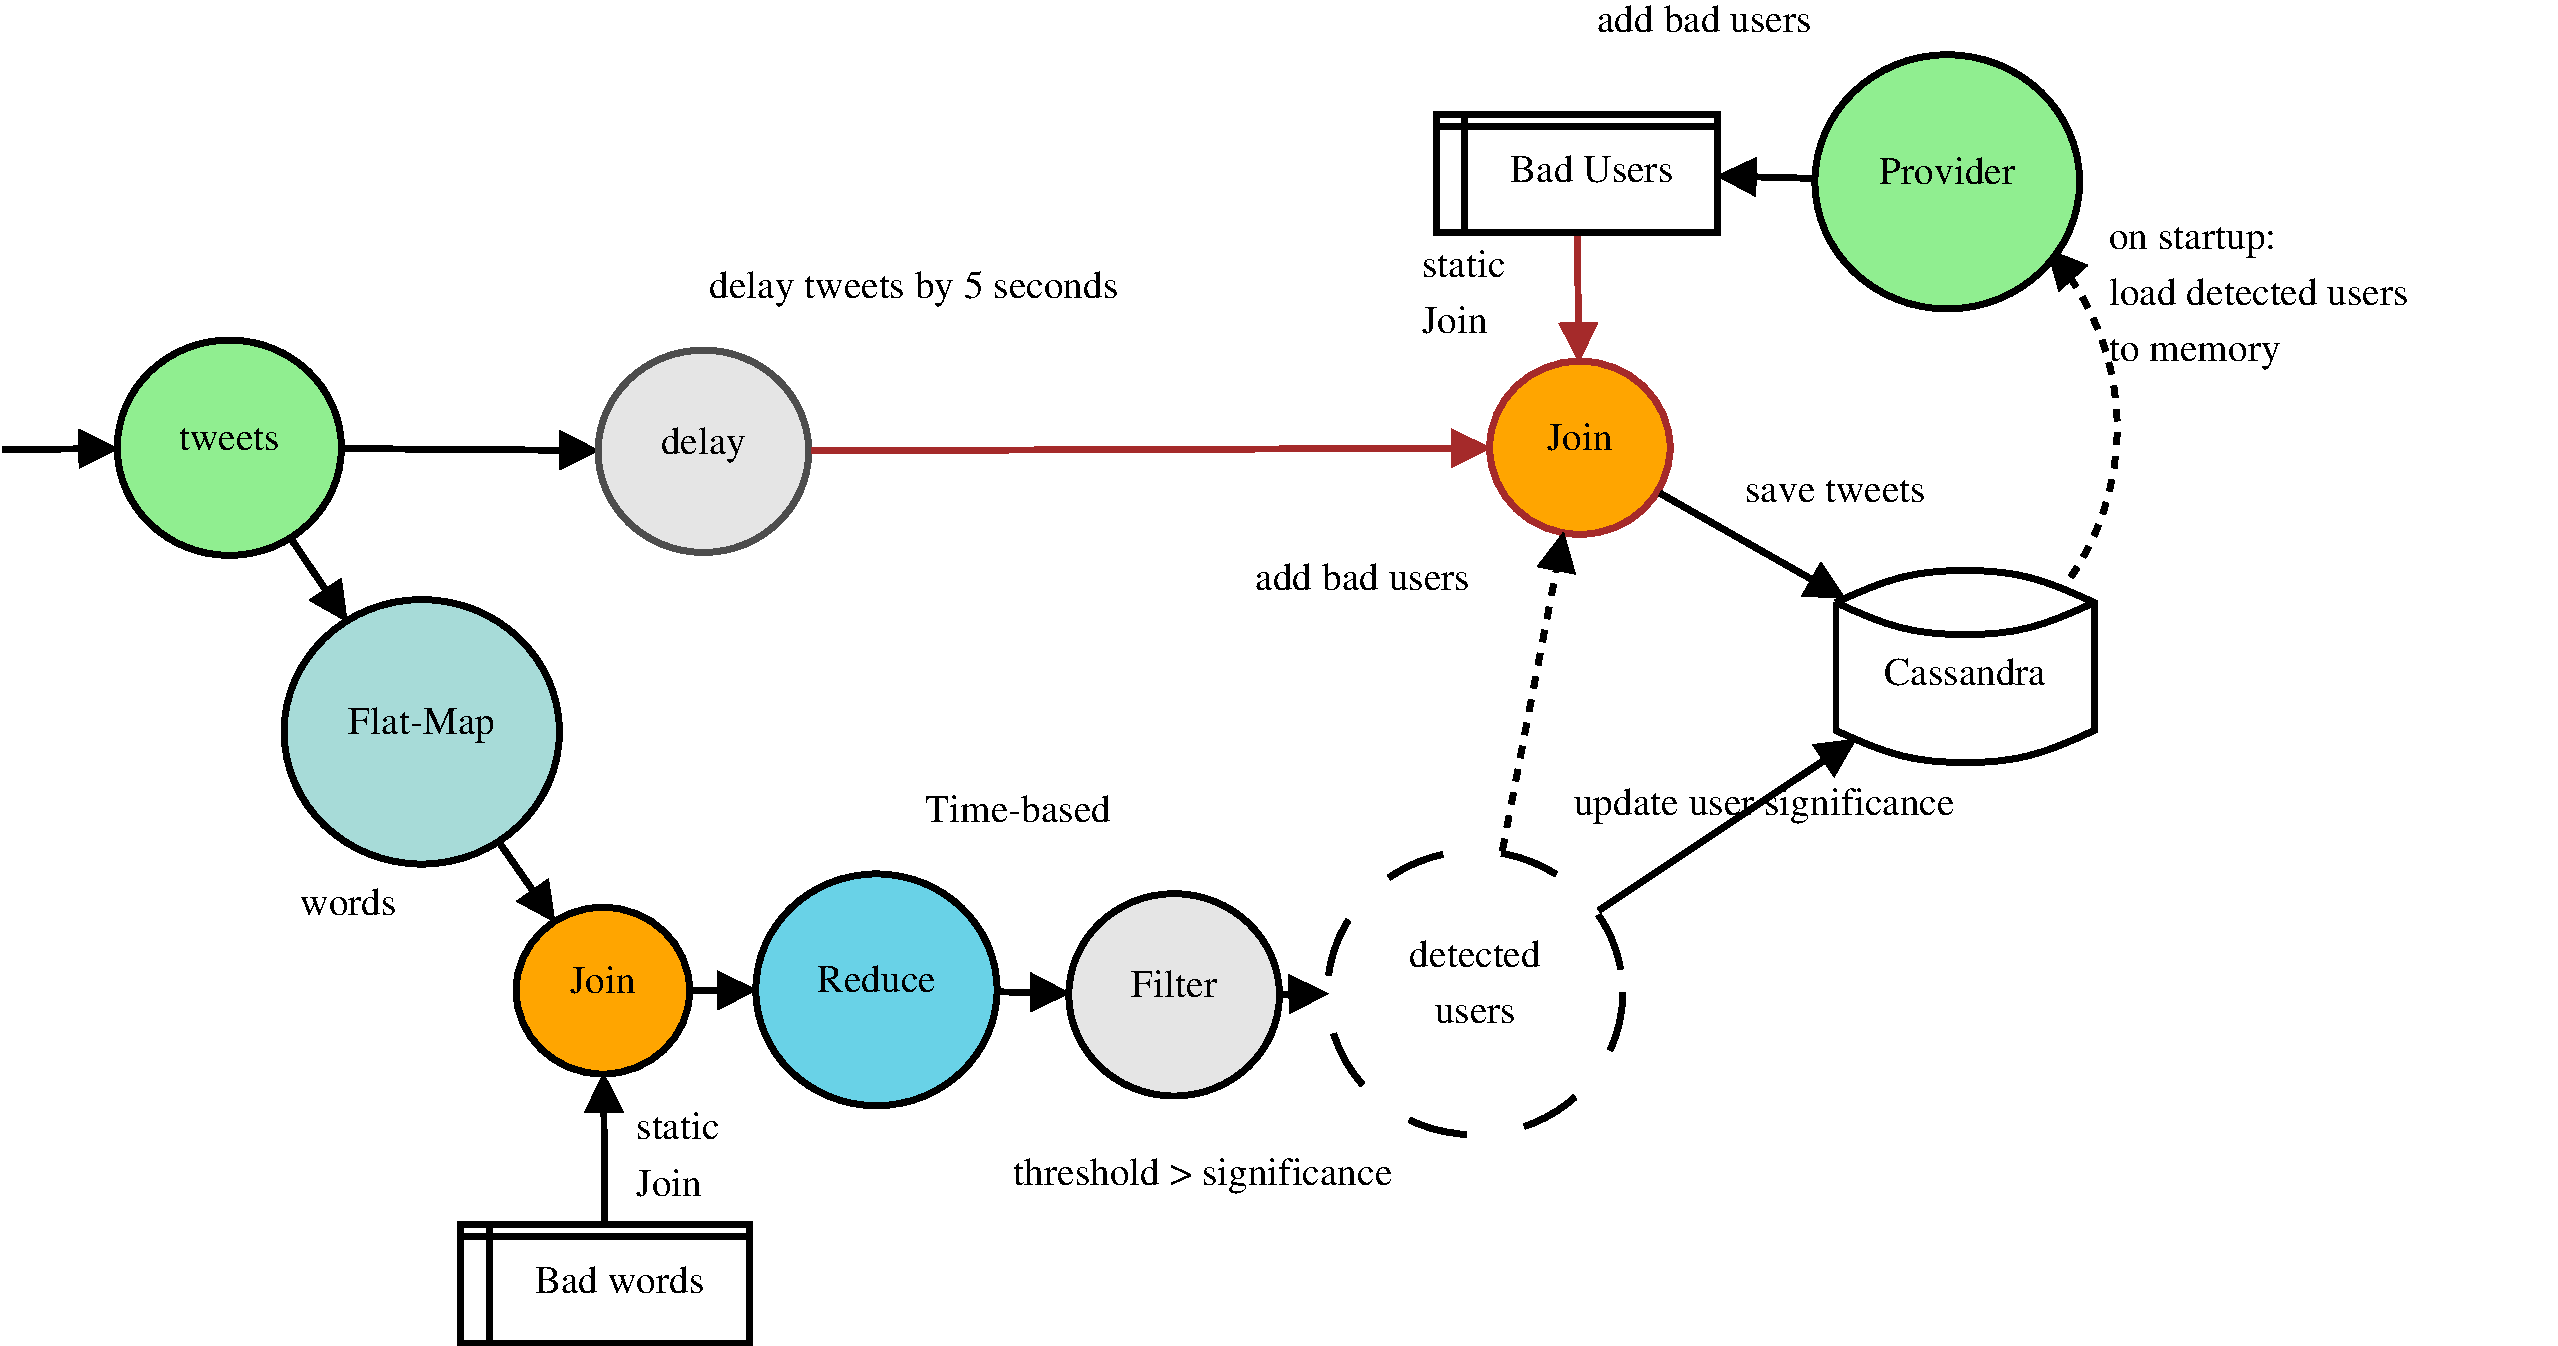
\includegraphics[width=0.55\textwidth]{images/AnalyzeTweetsTopology-eps-converted-to.pdf}
  \caption{This figure shows operators used in the topology and how they are related to each other. Operators are depicted as filled circles, in-memory storage is depicted as rectangles and dotted circles describe outputs within an operator for clarification.}
\end{figure}

\subsection{Topology}

The following section describe the topology used to the project use-case. The topology is divided two different streams orginated at the twitter stream source. The upper stream hold the tweets inside the topology until the second stream has analyzed the tweets and detected significanct users and inform the upper stream if it should skip or store tweets.

\subsubsection{Stream 1: Analyze Tweets}
\begin{description}
  \item[flatmap] \hfill \\
      Splits a whole tweet into single words and emit these words
      \newline output: \texttt{[Word,TweetId,User]}
  
  \item[join] \hfill \\
      Given is list of bad words. These bad words are joined with each of the words and emited with a predefined bad-word significance.
      \newline output: \texttt{[BadWord,TweetId,User,significance]}
  \item[reduce] \hfill \\
      The reducer compute the total-significance for a tweet. Each Bolt has to group the incoming tuples by \newline \texttt{[TweetId,User]}. The total-significance is computed a multiplication of all bad word occurences in a tweet.
      \newline output: \texttt{[TweetId,User,total-significance]}
      
  \item[filter] \hfill \\
      This filter operator allows to filter tweets above a specific significance threshold. In this Use-Case we set this to 1 to process all bad-words from users. The result are new detected users which are forwarded to the join operator of Stream 1 holding the tweets.

  \item[detected users] \hfill \\
      This dottet bolt is only to show the result of the whole stream. Detected users are forwarded to the join operator of Stream 1 holding the tweets. This needs a distinct tuple processing of incoming tuples from different sources. 
      
\end{description}

\subsubsection{Stream 2: Hold tweets}
\begin{description}
  \item[delay] \hfill \\
      The stream is orginated the the tweet stream source depicted in figure as an green node. The delayed bolt only hold the tweets for a specific time inside the topology until the tweets has been analyzed. The output is the same as the input.

  \item[join] \hfill \\
	The join operator received delayed tweet which are join with an in-memory hashtable containing detected users.
\end{description}

\subsection{Cassandra sink}
The cassandra sink operator takes care storing incoming tuples into cassandra tables. The operator analyze the incoming tuples, create new data structures if not exists and store theses tuples. The cassandra sink operator supports two different modes
\begin{description}
  \item[non-counter mode] \hfill \\
	The cassandra operator receives a specific key list and field-list which are stored persistently 
  \item[counter-mode] \hfill \\
       The counter-mode allows to increment fields by a specifc value located by initial key-fields.
\end{description}


\subsection{Cassandra provider}

The cassandra provider is only used if the topology is shut down and restarts again. The total user-significance is stored in cassandra and is reloaded to keep this in-memory to allow real-time processing. As an initial processing the cassandra-provider read all detected users with its significance and forwarded to the join operator. 

\subsection{Cassandra schema}
As an persistent storage cassandra is used to store detected users with its significance and their tweets. The cassandra-operator supports two different modes how to store data into the database. The \keyword{no-counter} mode assigns a specific primary-key to the incoming tuples an puts into a table. The \keyword{counter} mode only allows the increment a specific coulmn field determined by a primary-key.  

\begin{description}
  \item[user\_significance] \textit{counter} \hfill \\
  This tables stores for each user its significance-level which is increased over time. This table contains two columns, the twitter \keyword{user} and its \keyword{significance}. This table is loaded into the topology after an crash or an cluster-restart happened.
  
  \item[user\_tweets] \textit{counter}  \hfill \\
  This table stores the tweets for each user. The primary-key is \keyword{user} and \keyword{tweet\_id} with fields \keyword{tweet}.
  
  \item[word\_count]  \textit{non-counter} \hfill \\
  This table counts word occurences of bad words resulting in an user-update. The table provide some overall statistics.
  
\end{description}
    
	\section{Topology-Setup}
\label{sect:topology}
	\section{Frontend}
\label{sect:frontend}
	\section{Infrastructure}
\label{sect:Infrastructure}
To run a Big-Data application, it is important to have a reliable underlying infrastructure. As cloud services matured over the past years, it is not reasonable to run Storm on a dedicated cluster.

We decided to use the \textsl{Amazon EC2} cloud, as we were already familiar with its usage and its capabilities, which perfectly met our demands, and we were also granted free access to it.

Using an out-of-the-box Storm, would surely have sufficed the needs of running the CIT-Storm topology, but it would have been inconvenient in its usage.

We developed a system of tools to manage the cluster and the submitted topologies in a comfortable and efficient way. This section describes, the different parts of CIT-Storm and how they play together.

\subsection{Storm cluster}
To set up a Storm cluster, three essential software components are needed:
\begin{itemize}
\item \textsl{Storm Nimbus}\\
The heart component of the Storm cluster. The Nimbus manages the starting and stopping of topologies and distributes the workload on all registered worker nodes.
\item \textsl{Storm Supervisor}\\
A Supervisor represents the worker in Storm. Every Supervisor has a defined number of independent worker processes, to use the CPU resources more efficient.
\item \textsl{Apache Zookeeper}
The Zookeeper has the task to coordinate and synchronize the cluster.
\end{itemize}

CIT-Storm enhances the collection of software needed, to serve its previously described purpose:

\begin{itemize}
\item \textsl{Apache Cassandra}\\
The Cassandra database is used to store the results created by the topology, such as filtered tweets, bad-words and user significance.
\item \textsl{MySQL}\\
MySQL is used as a multi-purpose tool to manage user accounts for CIT-Storm access, store logs created by the Supervisors and to hold the IP-addresses of all connected cluster instances.
\item \textsl{Play-Framwork}\\
The web-frontend is created using the Play-Framework.
\end{itemize}

Now, that all software components are determined, they must be assigned to different EC2 instances.

\subsection{EC2 instances}
To have a dynamic cluster setup it is necessary to identify the roles of all server types in order to install the software and then bundle the system as a bootable instance image.\\

When developing CIT-Storm, a cluster setup with four different instance types appeared to be ideal.

\begin{description}
\descriptor{CIT-Storm Main Server}
A central server is needed to provide controls for the CIT-Storm system. In our case, the main server is an always-on instance with a static IP-address, so it can always be addressed the same way. To make the work with CIT-Storm even more convenient, we registered a domain-name at TwoDNS, to make it accessible via:\\
\texttt{http://citstorm.dd-dns.de}

The central server hosts the MySQL database, and the web-frontend, as well as the Zookeeper. In Storm, every node must be configured via a configuration file called \texttt{storm.yaml}, which is loaded when Storm starts. As the main server has a static IP-address, it can be hard coded in the storm configuration for the Zookeeper.

Unfortunately, the IP-addresses of the other servers are unknown, as they are dynamically determined by Amazon. To obtain and remember them, the Zookeeper could be used, as it provides a naming service. For our project, we decided to develop a compact naming server, as using the Zookeeper would cause overhead for a small sized cluster.\\
Our naming service is written in Java and uses an embedded Jetty web-server to enable REST-based access. Once a server is started, it registers itself at the naming server by using the relative url:\\
\texttt{/register?type=server-type},
where \texttt{server-type} can be one of the following roles \texttt{nimbus}, \texttt{supervisor} and \texttt{cassandra}.\\
Once the server receives the GET-request, it saves the requesters IP-address along with the server-type to the MySQL database. When a server needs information about the addresses of the other instances, it can call it with the GET-request: \texttt{/lookup?type=server-type}. The server responds either with a single IP-address, as for the Nimbus and Cassandra server, or with a comma-separated-list of IP-addresses for the Supervisors, as there can be more than one of them.\\
In the background, a timed thread checks recurrently, if the registered instances are still reachable and, if not, deletes them from the database.

The main server also starts up the cluster and in order to do so, it must have access to the Amazon Web Services (AWS). Amazon provides a set of tools to control EC2 instances from a console. These tools, called Amazon AWS Command Line Interface tools, can start and stop instances in EC2 and also request information about all running instances and their current state. The result is printed on the console in the JSON format, and can be processed from there. We wrote a Java program, that can start and stop instances by running the AWS CLI tools with a process builder. This program is accessed by the web-frontend to manage the cluster.

\descriptor{Nimbus}
The Nimbus instance runs the Storm Nimbus software, as well as a web-interface provided by Storm, the Storm UI. It can be used to observe the cluster, as well as the running topologies.

As our goal was it to make the use of Storm convenient, a method was needed, to store the topologies on the nimbus and start the topology, without hacking cryptic commands on a SSH-terminal. So, we developed a software, that offers a service to upload a file onto the Nimbus and to run and kill a topology. The program is written in Java and uses an embedded Jetty web-server to provide a REST-based web-service.

Using a POST-request, a file can be uploaded to the server using this URL (relative to the base URL of the Nimbus): \texttt{/upload}.\\
The server returns a unique-file-identifier, which can be used to start and stop the topology stored in the file, or to delete it from the Nimbus. The relative URLs to perform these actions are:\\
\texttt{/delete?file=filename}\\
\texttt{/run?file=filename\&name=topology-name}\\
\texttt{/kill?file=filename}

\descriptor{Supervisor}
The Supervisor instance only runs the Storm Supervisor, to dedicate all its resources to running the topologies.\\
When the Supervisor starts up, the configuration file needs to be adapted, as the Nimbus IP-address is unknown at the time of the creation of the instance image. As the main server provides a naming server for all involved machines, the configuration on the Supervisor is rewritten every time it starts up, using the current IP-address of the nimbus.

\descriptor{Cassandra}
Although the Cassandra database is not updated very frequently, it is installed on a separate EC2 instance, to maintain the possibility of extending the database, whether to a larger instance, or even to a Cassandra cluster,

\end{description}
	\section{Testing}
\label{sect:testing}

	As a distributed topology in a Big-Data environment could be a complex structure, testing is (as always) no marginal problem. In our Storm based scenario, we have Spouts that are emitting the initial input into the topology, Bolts that are executing operations on that input in one or several chains of neighbouring Bolts and we have the topology that combines Spouts and Bolt chains with each other to form a structure, which is able to solve a specific Big-Data analytics problem. 
	In such a scenario, it is not easy to find and solve problems and errors, as monitoring is only in place for the whole topology and not for each individual element. Additionally, a Storm topology is only debuggable at runtime, which makes it quite hard to find bugs or \textit{at least just realize that the topology is not working as expected} for large setups. 
	To find problems and errors in such a setup several points of view are needed to be addressed in order to find the source of a problem faster and more reliable as it would usually be the case.
	
\subsection{Test-Suite Approach}
	In order to cope with the challenges of testing in complex and distributed Storm environments, we developed our own Test-Suite, which focuses on three different levels that may contain, combined with each other, the most common problem sources in an instance of one of our CIT-Storm topologies. The three different problem levels that we considered of importance were the following ones, sorted by abstraction level in the topology:
	
	\begin{description}
	 \descriptor{Operator-Tests}
		Are describing the validity of a specific user defined function that is caring about the input tuple execution inside a Bolt. For a well defined testing setup, each Bolt inside the testing topology should have an Operator- \& a Bolt-Test (described beneath) to fully assure that the respective Bolt is behaving as expected \textit{without any outside influences}, namely predecessor Bolts that are sending unexpected input to this Bolt. An Operator-Test is thus using pre-defined tuple input and checks if the asserted output of the operator to be tested is matching with the factual output.
		\begin{center}
			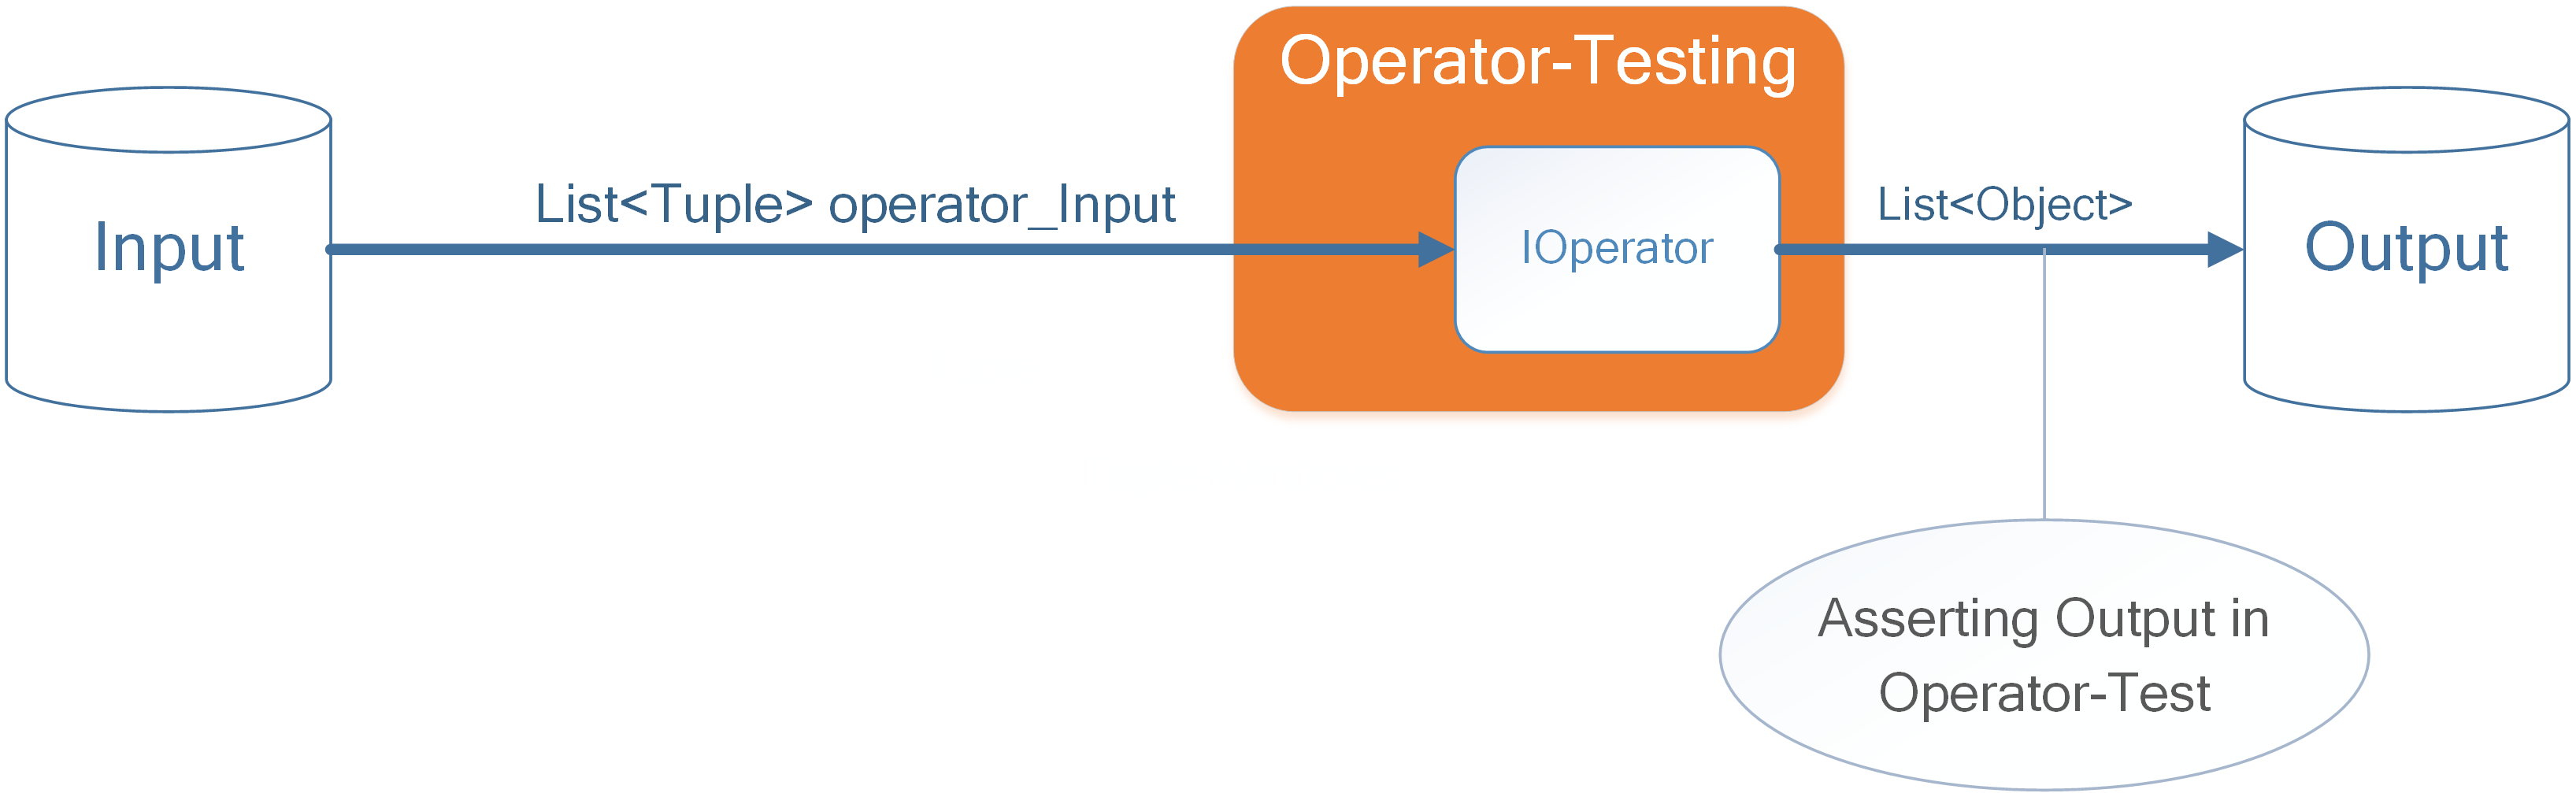
\includegraphics[width=0.4\textwidth]{./images/08_testing/OperatorTests.png}
		\end{center}

		
	 \descriptor{Bolt-Tests}
		Are combining Operator-Tests with additional Window-Handling, as needed to build streaming input execution. In our CIT-Storm implementation (as defined in \ref{sect:udfBolt}), we are using \textit{Time-} or \textit{Count-Windows} to wait a specific time or for a specific amount of input tuples, until the execution of those input tuples will be passed to the Operator. \\
		In perspective if this Testing-Suite, the Operator-Test (which was already successfully executed before) is only returning the correctness of a given input, relative to an asserted output, whereas a Bolt-Test includes testing with focus on the used window and its output after a \texttt{window.flush()}. The Bolt-Test will only be successful when a window returns the expected tuples after a given time and the Operator will correctly handle this input.
		\begin{center}
			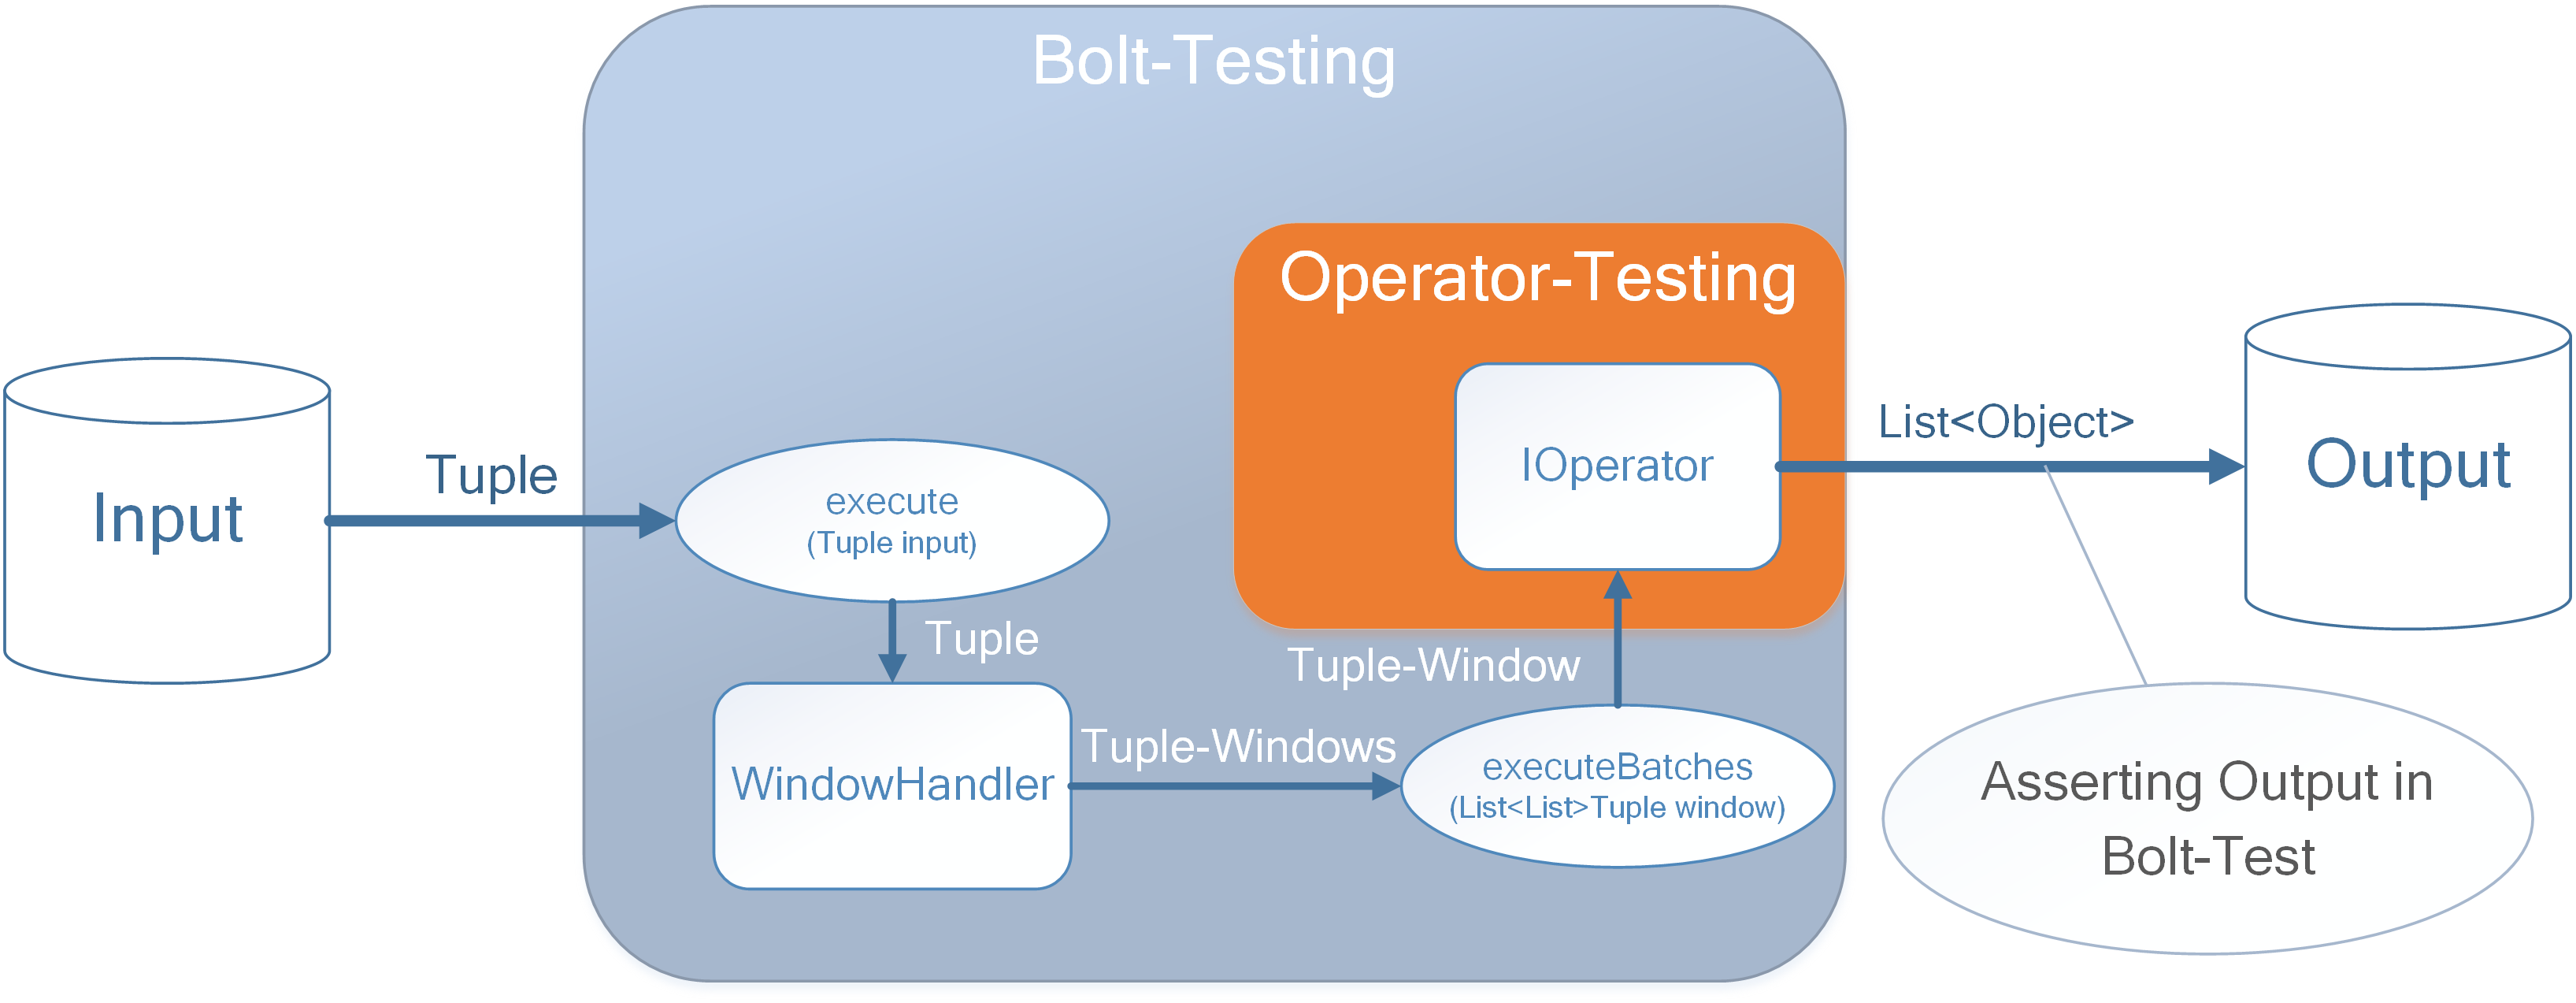
\includegraphics[width=0.4\textwidth]{./images/08_testing/BoltTests.png}
		\end{center}
	 
	 \descriptor{Topology-Tests}
		In order to test the topology as a whole, the Test-Suite provides a test skeleton named \texttt{TopologyTest}. A specific TopologyTest-Scenario is inherited by this class and allows the test-designer to test \textit{chains of Bolts with a Spout as source} in one run. Of course, this is not handling the complexity that Storm could cope with in its topologies, but as the Test-Suite is running outside a Storm environment (more on the implementation details may be found in the upcoming section \ref{sect:TestSuiteRealization}), it would be a likewise complex (and error-prone) task to completely simulate every aspect of Storm.\\
		The Topology-Test however does focus on linear topologies, which is describing most of the regular use-cases inside a Big-Data scenario. Even if the real Storm topology would use different Stream-Groupings (described in \ref{sect:StreamGroupings} on page \pageref{StreamGroupings}), the shuffled topology input could mostly be baked onto a linear topology. \\
		In order to set up a TopologyTest, import each Bolt from the topology to be tested into the test-class's \texttt{defineTopologySetup()} and add the respective Bolt in a \texttt{BoltTestConfig} in the order you want them to be placed in the testing chain. Each \texttt{BoltTestConfig} is carrying the respective \texttt{UDFBolt}, a Bolt-TestName, a timeout per tuple input (needed for \texttt{TimeWindows}) and an assertedOutput with it, in order to fully define a TopologyTest. The test run is then defined as an execution of different Bolt-Tests, initialized by the different \texttt{BoltTestConfigs}. Each Bolt-Test receives the output of the predecessing Bolt-Test as its own input. A Topology-Test could thus only succeed, if each Bolt-Test (and the Operator-Tests inside those) succeeds and on top of that, if the final output matches with the final asserted output of the topology, respective to the initial input.
		
		
	\end{description}

\subsection{Test-Suite Realization}
\label{sect:TestSuiteRealization}
	

\subsection{Treated Use-Cases}
\label{sect:TestSuiteUseCases}
	

\subsection{Test-Suite Limitations}
\label{sect:TestSuiteLimitations}
	
	\section{Conclusion}
\label{sect:conclusion}
	
	%\thebibliography{References}
	\printbibliography
\end{document}
